\usetikzlibrary{arrows.meta}
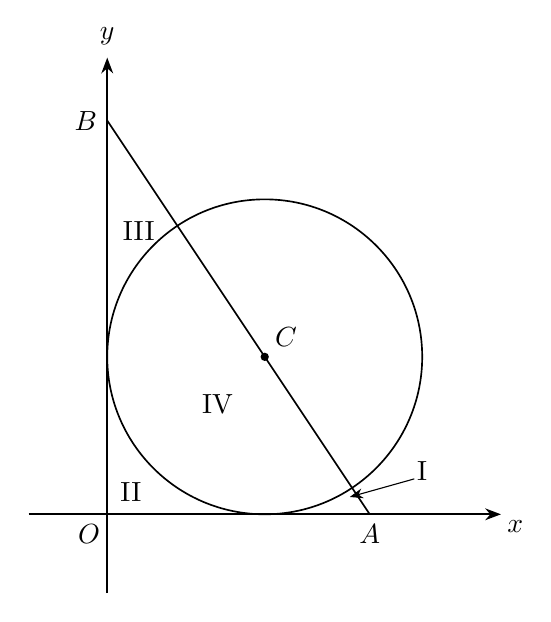
\begin{tikzpicture}[x=1cm,y=1cm,line width=.6pt,font=\normalsize,>=Stealth]
\coordinate (O) at (0,0);
\coordinate (C) at (2,2);
\coordinate (A) at (3.333333,0);
\coordinate (B) at (0,5);
\draw[->] (-1,0)--(5,0);
\draw[->] (0,-1)--(0,5.8);
\draw (C) circle[radius=2];
\draw (A)--(B);
\fill (C) circle[radius=1.5pt];
\node[anchor=north east,inner sep=0pt] at (-0.08,-0.12) {$O$};
\node[anchor=north,inner sep=0pt] at (3.333333,-0.12) {$A$};
\node[anchor=east,inner sep=0pt] at (-0.12,5) {$B$};
\node[anchor=south west,inner sep=0pt] at (2.12,2.12) {$C$};
\node[anchor=north west,inner sep=0pt,xshift=2pt,yshift=-2pt] at (5.0,0.0) {$x$};
\node[anchor=south,inner sep=0pt] at (0,5.95) {$y$};
\node[inner sep=0pt] at (0.3,0.28) {II};
\node[inner sep=0pt] at (0.4,3.6) {III};
\node[inner sep=0pt] at (1.4,1.4) {IV};
\node[inner sep=0pt] at (4,0.55) {I};
\draw[->,line width=.4pt] (3.9,0.45)--(3.08,0.22);
\end{tikzpicture}
